\documentclass[a4paper,10pt]{article}
\usepackage[utf8]{inputenc}

\usepackage{a4wide}
\usepackage{cite}
\usepackage{hyperref}
\usepackage[pdftex]{graphicx}
\usepackage{url}

\usepackage[english]{babel}
\usepackage{caption}
\usepackage{amsmath}
\usepackage{listings}

\usepackage[parfill]{parskip}

%opening
\title{My solution for the Galaxy Zoo challenge}
\author{Sander Dieleman}


\begin{document}

\maketitle

\begin{abstract}
This document describes my solution for the Galaxy Challenge on Kaggle. I had previously documented my solution in a blog post\footnote{\url{http://benanne.github.io/2014/04/05/galaxy-zoo.html}}. Many parts of this document are taken from that post. This document additionally provides information on how to use the code, which has been made publicly available under a BSD 3-clause licence in accordance with the requirements for prize eligibility.
\end{abstract}

\section*{Personal details}

\begin{itemize}
 \item{Name:} Sander Dieleman
 \item{Location:} Ghent, Belgium
 \item{Email:} \href{mailto:sanderdieleman@gmail.com}{sanderdieleman@gmail.com}
 \item{Competition:} Galaxy Zoo - The Galaxy Challenge\footnote{\url{http://www.kaggle.com/c/galaxy-zoo-the-galaxy-challenge}}
\end{itemize}

\tableofcontents

\section{Summary}

My solution is based around \textit{convolutional neural networks} (convnets). I used fairly large models (the largest network has about 42 million parameters) with 5 to 7 layers, and as a result my main focus during the competition was combatting overfitting. I did this by using data augmentation (creating new datapoints from existing datapoints by transformations which the target values should be invariant to), dropout and weight norm constraints, and modifying the network architecture to increase parameter sharing. I trained all networks with stochastic gradient descent with Nesterov momentum and used GPU acceleration to speed up experiments. My final submission was an ensemble of 17 models, which differed in architecture and input preprocessing. No external data sources were used.


\section{Models and training}

\subsection{Preprocessing and data augmentation}

\subsubsection{Cropping and downsampling}

The data consisted of 424x424 colour JPEG images, along with 37 weighted probabilities that have to be predicted for each image\footnote{for details on the weighting scheme, please refer to \url{http://www.kaggle.com/c/galaxy-zoo-the-galaxy-challenge/details/the-galaxy-zoo-decision-tree}.}. For almost all of the images, the interesting part was in the center, so I cropped all images to 207x207. I then downsampled them 3x to 69x69, to keep the input size of the network manageable.

\subsubsection{Exploiting spatial invariances}

Images of galaxies are rotation invariant. They are also scale invariant and translation invariant to a limited extent. All of these invariances could be exploited to do data augmentation. Each training example was perturbed before presenting it to the network by randomly scaling it, rotating it, translating it and optionally flipping it. I used the following parameter ranges:

\begin{itemize}
 \item{rotation:} random with angle between 0$^\circ$ and 360$^\circ$ (uniform)
 \item{translation:} random with shift between -4 and 4 pixels (relative to the original image size of 424x424) in the x and y direction (uniform)
 \item{zoom:} random with scale factor between 1/1.3 and 1.3 (log-uniform)
 \item{flip:} yes or no (bernoulli)
\end{itemize}

Because both the initial downsampling to 69x69 and the random perturbation are affine transforms, they could be combined into one affine transformation step. This sped up things significantly and reduced information loss.

\subsubsection{Colour perturbation}
\label{sec:colour-perturbation}
After this, the colour of the images was changed as described by Krizhevsky et al. \cite{Krizhevsky2012}, with two differences: the first component had a much larger eigenvalue than the other two, so only this one was used, and the standard deviation for the scale factor alpha was set to 0.5.

\subsubsection{`Realtime' augmentation}

Combining downsampling and perturbation into a single affine transform made it possible to do data augmentation in realtime, i.e. during training. This significantly reduced overfitting because the network would never see the exact same image twice. While the network was being trained on a chunk of data on the GPU, the next chunk would be generated on the CPU in multiple processes, to ensure that all the available cores were used.

\subsubsection{Centering and rescaling}

I experimented with centering and rescaling the galaxy images based on parameters extracted with \textit{sextractor}\footnote{\url{https://www.astromatic.net/software/sextractor}}. Although this didn't improve performance, including a few models that used it in the final ensemble helped to increase variance. I extracted the center of the galaxies, as well as the \emph{Petrosian radius}. I then centered each image by shifting the estimated center pixel to (212, 212), and rescaled it so that its Petrosian radius would be equal to 160 pixels. The scale factor was limited to the range (1/1.5, 1.5), because there were some outliers. This rescaling and centering could also be collapsed into the affine transform doing downsampling and perturbation, so it did not slow things down at all.

\subsection{Model architecture}

\subsubsection{Exploiting rotation invariance}
\label{sec:exploiting-rotation-invariance}
I increased parameter sharing in the network by cutting the galaxy images into multiple parts that could be treated in the same fashion, i.e. processed by the same convolutional architecture. For this I exploited the rotation invariance of the images. As mentioned before, the images were cropped to 207x207 and downsampled by a factor of 3. This was done with two different orientations: a regular crop, as well as one that is rotated 45$^\circ$. Both of these crops were also flipped horizontally, resulting in four 69x69 `views' of the image. This is visualised in Figure \ref{fig:schema-views}.

\begin{figure}
        \centering
	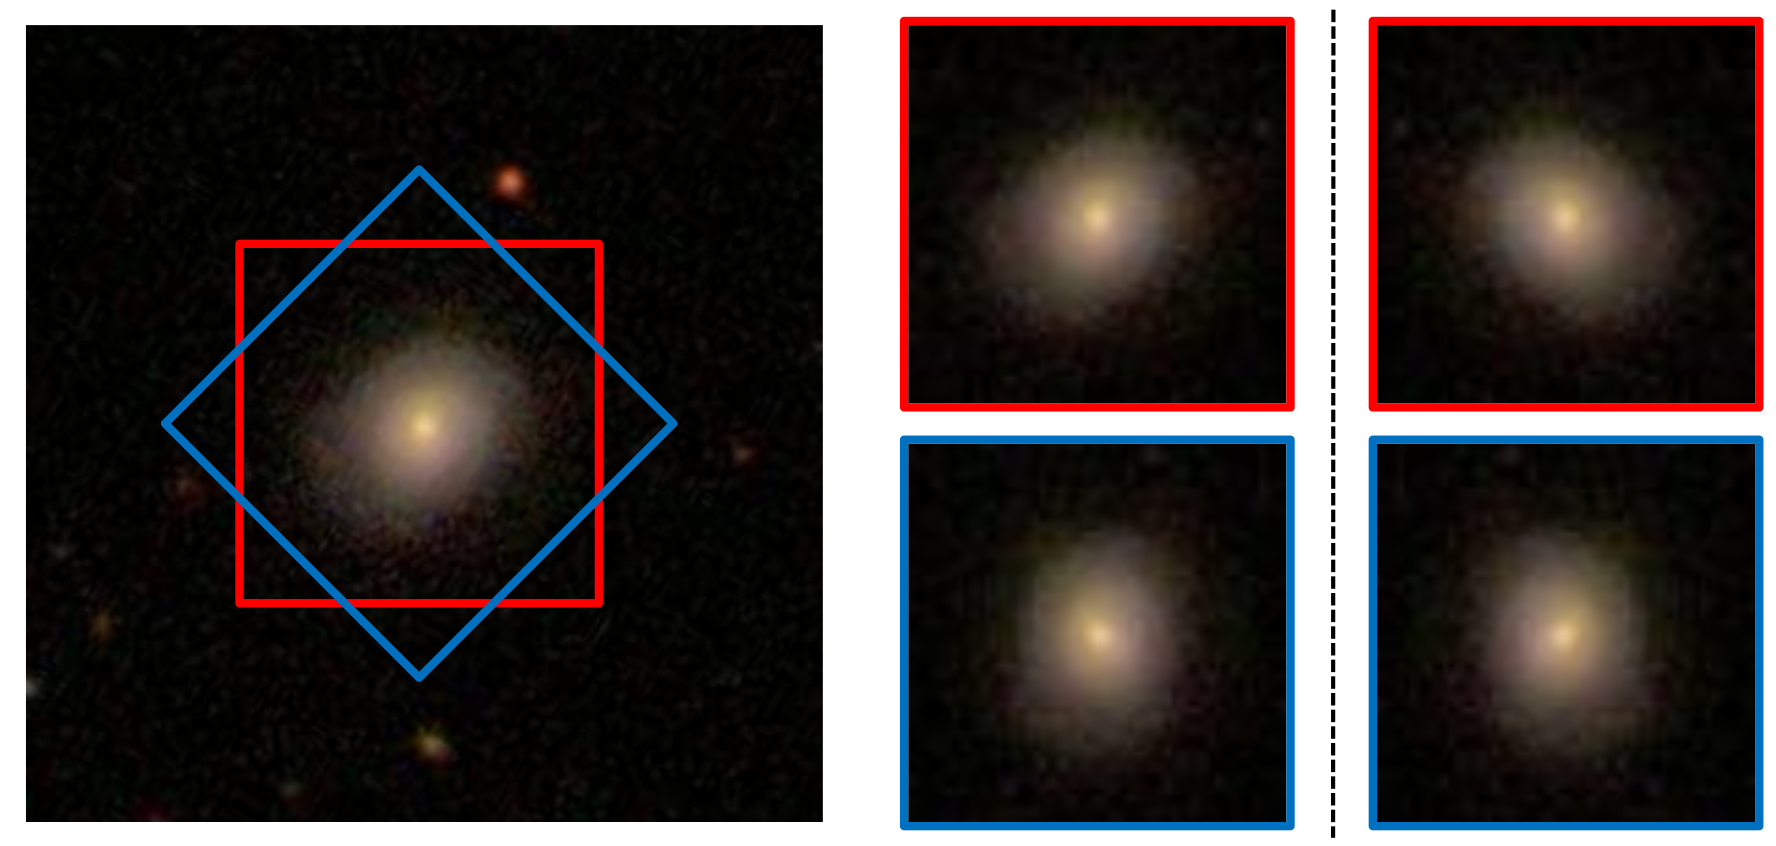
\includegraphics[width=0.8\textwidth]{schema_views.png}
        \caption{Four different \textit{views} were extracted from each image: a regular view (red), a 45$^\circ$ rotated view (blue), and mirrored versions of both.}\label{fig:schema-views}
\end{figure}


Each of the four views was again split into four partially overlapping `parts' of size 45x45. Each part was rotated so that they are all aligned, with the galaxy in the bottom right corner. This is visualised in Figure \ref{fig:schema-parts}. In total, 16 parts were extracted from the original image.

\begin{figure}
        \centering
	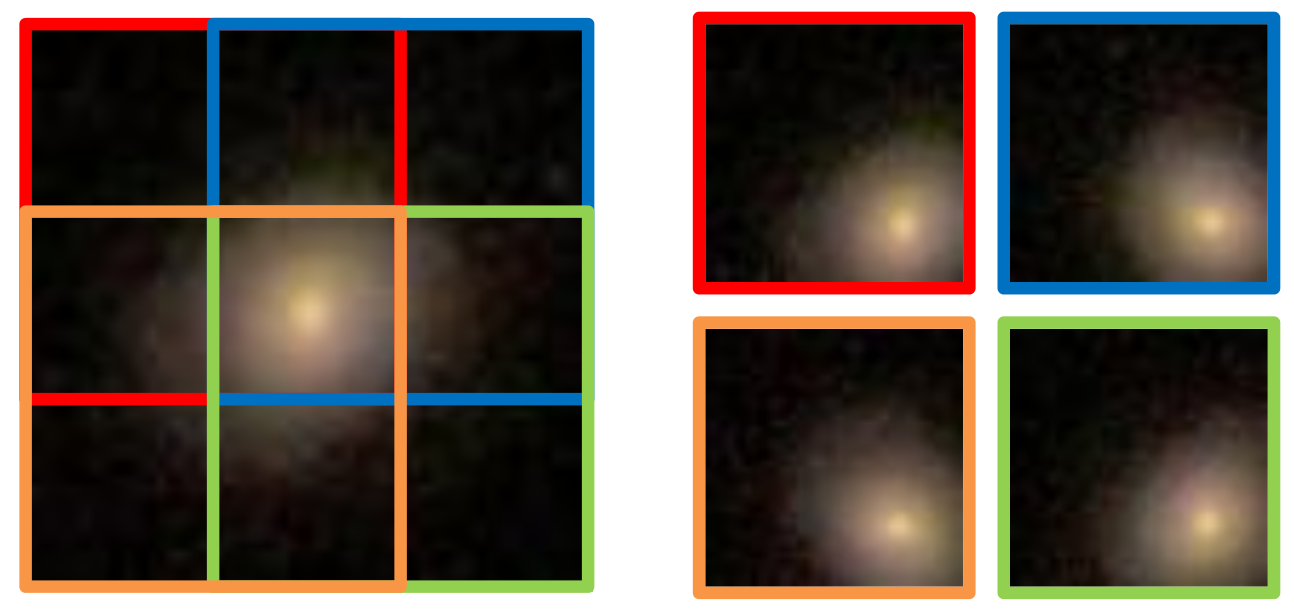
\includegraphics[width=0.8\textwidth]{schema_parts.png}
        \caption{Each view was then split into four partially overlapping \textit{parts}. Each part was rotated so that they are all aligned, with the galaxy in the bottom right corner. In total, 16 parts were extracted from the original image.}\label{fig:schema-views}
\end{figure}

This results in 16 smaller 45x45 images which appear very similar. They can be expected to have the same topological structure due to rotation invariance, so they can be processed by the same convolutional architecture, which results in a 16x increase in parameter sharing, and thus less overfitting. At the top of the network, the features extracted from these 16 parts are concatenated and connected to one or more dense layers, so the information can be aggregated.
 
Due to the overlap of the parts, a lot of information is available about the center of the galaxy, because it is processed by the convnet in 16 different orientations. This is useful because a few important properties of the galaxies are expected to be in the center of the image (the presence of a bar or a bulge, for example). Reducing this overlap typically resulted in reduced performance. I chose not to make the parts fully overlap, because it would slow down training too much.

\subsubsection{Incorporating output constraints}
\label{sec:output-constraints}
The 37 outputs to be predicted are weighted probabilities, adhering to a number of constraints. Incorporating these constraints into the model turned out to be beneficial. In essence, the answers to each question should form a categorical distribution. Additionally, they are scaled by the probability of the question being asked, i.e. the total probability of answers given that would lead to this question being asked.

Using a softmax output for each question, and then applying the scaling factors didn't make much of a difference. I believe this is because the softmax function has difficulty predicting hard zeros and ones, of which there were quite a few in the training data (its input would have to be very large in magnitude).

In the end I normalised the distribution for each question by adding a rectification nonlinearity in the top layer instead of the softmax functions, and then just using divisive normalisation. For example, if the raw, linear outputs of the top layer of the network for question one were $z_1, z_2, z_3$, then the actual output for question one, answer one was given by:
\begin{equation}
y_1 = \dfrac{\max(z_1, 0)}{\max(z_1, 0) + \max(z_2, 0) + \max(z_3, 0) + \epsilon},
\end{equation}
where $\epsilon$ is a very small constant that prevented division by zero errors. I set it to 1e-12. This approach allowed the network to predict hard zeros more easily.

\subsubsection{Architecture of the best model}

The best model I found is shown in Figure \ref{fig:architecture} in the form of a Krizhevsky-style diagram. All other models included in the final ensemble I submitted are slight variations of this model.

\begin{figure}
        \centering
	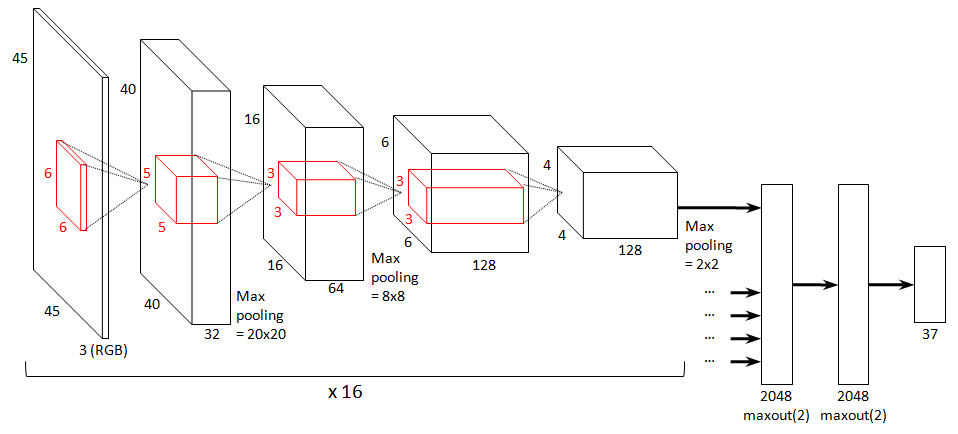
\includegraphics[width=1.0\textwidth]{architecture.png}
        \caption{Krizhevsky-style diagram of the architecture of the best performing network.}\label{fig:architecture}
\end{figure}

The input is presented to the model in the form of RGB coloured 45x45 image parts. The model has 7 layers: 4 convolutional layers and 3 dense layers. All convolutional layers include a ReLU nonlinearity (i.e. $f(x) = \max(x, 0)$). The first, second and fourth convolutional layers are followed by 2x2 max-pooling. The sizes of the layers, as well as the sizes of the filters, are indicated in the figure.

As mentioned before, the convolutional part of the network is applied to 16 different parts of the input image. The extracted features for all these parts are then aggregated and connected to the dense part of the network. The dense part consists of two maxout layers with 2048 units \cite{goodfellow2013maxout}, both of which take the maximum over pairs of linear filters (so 4096 linear filters in total). Using maxout here instead of regular dense layers with ReLUs helped to reduce overfitting a lot, compared to dense layers with 4096 linear filters. Using maxout in the convolutional part of the network as well proved too computationally intensive. Training this model took 67 hours on the available hardware (see Section \ref{sec:dependencies}).

\subsubsection{Variants}
\label{sec:variants}

Variants of the best model were included in the final ensemble I submitted, to increase variance (see Section \ref{sec:model-averaging}). They include:

\begin{itemize}
 \item a network with two dense layers instead of three (just one maxout layer);
 \item a network with one of the dense layers reduced in size and applied individually to each part (resulting in 16-way parameter sharing for this layer as well);
 \item a network with a different filter size configuration: 8/4/3/3 instead of 6/5/3/3 (from bottom to top);
 \item a network with centered and rescaled input images;
 \item a network with a ReLU dense layer instead of maxout;
 \item a network with 192 filters instead of 128 for the topmost convolutional layer;
 \item a network with 256 filters instead of 128 for the topmost convolutional layer;
 \item a network with norm constraint regularisation applied to the two maxout layers (as in Hinton et al. \cite{Hinton2012});
 \item combinations of the above variations.
\end{itemize}

\subsection{Training}

\subsubsection{Validation}

For validation purposes, I split the training set in two parts. I used the first 90\% for training, and the remainder for validation. Near the end of the competition I tried retraining a model on the entire training set, including the validation data I split off, but I noticed no increase in performance on the public leaderboard, so I left it at that.

\subsubsection{Training algorithm}

I trained the networks with stochastic gradient descent (SGD) and Nesterov momentum (with a fixed momentum constant of 0.9). I used a minibatch size of 16 examples. This meant that the effective minibatch size for the convolutional part was 256, because each training image is split into 16 parts (see Section \ref{sec:exploiting-rotation-invariance}).

The training data was processed into \textit{chunks} of 10000 examples (one chunk was loaded into GPU memory at a time), so each chunk contained 625 minibatches. I trained the networks for 2500 chunks. I used a learning rate schedule with two discrete decreases. Initially it was set to 0.04. It was decreased tenfold to 0.004 after 1800 chunks, and again to 0.0004 after 2300 chunks. For the last few models I trained, the number of chunks was slightly decreased to 2100 to be able to finish training before the competition deadline.

For the first chunk, the divisive normalisation in the output layer described in Section \ref{sec:output-constraints} was disabled. This was necessary to ensure convergence (otherwise it would get stuck at the start sometimes).

\subsubsection{Initialisation}

Some fiddling with the parameter initialisation was required to get the network to train properly. Most of the layer weights were initialised from a Gaussian distribution with mean zero and a standard deviation of 0.01, with biases initialised to 0.1. For the topmost convolutional layer, I increased the standard deviation to 0.1. For the dense layers, I reduced it to 0.001 and the biases were initialised to 0.01. These modifications were necessary presumably because these layers are much smaller resp. bigger than the others.

\subsubsection{Regularisation}
Dropout was used in all three dense layers, with a dropout probability of 0.5. Near the very end of the competition I also experimented with norm constraint regularisation for the maxout layers. I chose the maximal norm for each layer based on a histogram of the norms of a network trained without norm constraint regularisation (I chose it so the tail of the histogram would be chopped off). I'm not entirely sure if this helped or not, since I was only able to do two runs with this setup.

\subsection{Model averaging}
\label{sec:model-averaging}

\subsubsection{Averaging across transformed images}

For each individual model, I computed predictions for 60 affine transformations of the test set images: a combination of 10 rotations, spaced by 36$^\circ$, 3 rescalings (with scale factors 1/1.2, 1 and 1.2) and flipping / no flipping. These were uniformly averaged. Even though the model architecture already incorporated a lot of invariances, this still helped quite a bit. Computing these averaged test set predictions for a single model took just over 4 hours.

\subsubsection{Averaging across architectures}

The averaged predictions for each model were then uniformly blended again, across a number of different models (variants of the model described in Section \ref{sec:variants}). I also experimented with a weighted blend, optimised on the validation set I split off, but this turned out not to make a significant difference. However, I did use the learned weights to identify sets of predictions that were not contributing at all, and I removed those from the uniform blend as well.

My final submission was a blend of predictions from 17 different models, each of which were themselves blended across 60 transformations of the input. So in the end, I blended 1020 predictions for each test set image.

For comparison: my best single model achieved a score of \textbf{0.07671} (public leaderboard) / \textbf{0.07693} (private leaderboard). After averaging across transformed images and architectures, I achieved a final score of \textbf{0.07467} (public) / \textbf{0.07492} (private).


\section{Code description}

This section describes the implementation. Please note that some of the published code was not used to generate the winning solution, and is not described here. I wanted to make it available anyway in case it proves useful for someone, and taking all the files apart to remove unused code would probably have introduced bugs. In addition, some methods are only used internally by other methods, and were left out of this description to avoid clutter.

\subsection{Relevant paths}
\label{sec:paths}
A number of paths are hardcoded, and the necessary files and directories need to be in place for some scripts to work. These paths are listed below. Section \ref{sec:generating} describes step by step where to place the downloaded data files and how to generate the other necessary files.

\begin{itemize}
 \item \path{data/}: contains all train and test data
 \item \path{data/raw/}: contains the data as it was provided on Kaggle
 \item \path{data/raw/training_solutions_rev1.csv}: the provided CSV file with training labels
 \item \path{data/raw/images_train_rev1/}: contains the train images in their original format (JPEG files)
 \item \path{data/raw/images_test_rev1/}: contains the test images in their original format (JPEG files)
 \item \path{/dev/shm/images_*_rev1/}: the JPEG files are copied to RAM (\path{/dev/shm} on Linux systems) for faster loading using \path{copy_data_to_shm.py}
 \item \path{data/solutions_train.npy}: train labels in a NumPy array, generated by \path{convert_training_labels_to_npy.py}
 \item \path{data/train_ids.npy}: ids of the train set in a NumPy array, generated by \path{create_train_ids_file.py}
 \item \path{data/test_ids.npy}: ids of the test set in a NumPy array, generated by \path{create_test_ids_file.py}
 \item \path{data/pysex_params_*.npy.gz}: these files contain parameters extracted from the image with sextractor. They are generated by \path{extract_pysex_params_extra.py} and \path{extract_pysex_params_gen2.py}.
 \item \path{analysis/final/*.pkl}: Python pickle files containing Python dictionaries with details about the training process, as well as final parameter values; created by running training scripts (\path{try_*.py})
 \item \path{predictions/final/*.csv.gz}: test set prediction files in CSV format, created by running training scripts (\path{try_*.py})
 \item \path{predictions/final/augmented/valid/*.npy.gz}: validation set prediction files in NumPy format, created by running augmented prediction scripts (\path{predict_augmented_npy_*.py}) (i.e. predictions averaged across transformed images)
 \item \path{predictions/final/augmented/test/*.npy.gz}: corresponding test set prediction files in NumPy format
 \item \path{predictions/final/blended/*.npy.gz}: test set prediction files in NumPy format containing predictions averaged across multiple architectures
\end{itemize}

\subsection{Python modules}

\subsubsection{Data loading: \texttt{load\_data.py}}

\paragraph{load\_data.train\_ids, .test\_ids:} NumPy arrays containing a list of image IDs for the train and test sets respectively.

\paragraph{load\_data.load\_image:} given an image ID, load a JPEG image from the dataset into a NumPy array and normalise it so all values are in the interval [0, 1].

Inputs:
 \begin{itemize}
  \item{img\_id:} the ID of the image.
  \item{subset='train':} the subset the image is part of ('train' or 'test').
  \item{normalise=True:} whether to normalise the values to [0, 1].
  \item{from\_ram=False:} load the image from \path{/dev/shm} instead of from \path{data/raw/}.
 \end{itemize}

Outputs:
\begin{itemize}
 \item{img:} a NumPy array with shape (424, 424, 3) containing the image data.
\end{itemize}

\paragraph{load\_data.load\_gz, .save\_gz:} extended versions of numpy.load and numpy.save that work with gzipped files.

\paragraph{load\_data.buffered\_gen\_mp:} generator that runs a slow source generator in a separate process. This is useful for doing data augmentation in parallel with training.

Inputs:
 \begin{itemize}
  \item{source\_gen:} the generator to run in a separate process.
  \item{buffer\_size=2:} the number of items to pre-generate and buffer.
  \item{sleep\_time=1:} number of seconds to sleep between attempts to get a new item from the buffer.
 \end{itemize}
 
\subsubsection{Realtime augmentation: \texttt{realtime\_augmentation.py}}

This module is usually imported as \path{ra} for convenience.

\paragraph{realtime\_augmentation.build\_ds\_transform:} creates a \path{skimage.transform.AffineTransform} object that represents a downsampling and cropping operation. Note that only the \path{ds_factor} and \path{target_size} arguments were used in most cases, the others were typically left to their default values.

Inputs:
 \begin{itemize}
  \item{ds\_factor=1.0:} the downsampling factor.
  \item{orig\_size=(424, 424):} tuple representing the original image size in pixels.
  \item{target\_size=(53, 53):} tuple representing the target size of the downsampled image in pixels.
  \item{do\_shift=True:} include a translation so the center part of the image is cropped.
  \item{subpixel\_shift=False:} if the downsampling factor is integer, enabling this will ensure that the pixel grid of the subsampled image is aligned with that of the original image.
 \end{itemize}
 
Outputs:
\begin{itemize}
 \item{tform\_ds:} a \path{skimage.transform.AffineTransform} object representing the downsampling and cropping operation.
\end{itemize}

\paragraph{realtime\_augmentation.build\_augmentation\_transform:} creates a \path{skimage.transform.AffineTransform} object that represents a data augmentation operation.

zoom=1.0, rotation=0, shear=0, translation=(0, 0)

Inputs:
 \begin{itemize}
  \item{zoom=1.0:} zoom factor.
  \item{rotation=0:} rotation angle in degrees.
  \item{shear=0:} shear angle in degrees.
  \item{translation=(0,0):} tuple representing the shift in the x and y directions in pixels.
 \end{itemize}
 
Outputs:
\begin{itemize}
 \item{tform\_augment:} a \path{skimage.transform.AffineTransform} object representing the data augmentation operation.
\end{itemize}

\paragraph{realtime\_augmentation.random\_perturbation\_transform:} creates a \path{skimage.transform.AffineTransform} object that representing a random dat augmentation operation.

Inputs:
 \begin{itemize}
  \item{zoom\_range:} range from which the zoom factor is sampled (log-uniform).
  \item{rotation\_range:} range (in degrees) from which the rotation angle is sampled (uniform).
  \item{shear\_range:} range (in degrees) from which the shear angle is sampled (uniform).
  \item{translation\_range:} range (in pixels) from which the shift in both the x and y directions is sampled.
  \item{do\_flip=False:} if True, a flip is incorporated into the transform half of the time (bernoulli).
 \end{itemize}
 
Outputs:
\begin{itemize}
 \item{tform\_augment:} a \path{skimage.transform.AffineTransform} object representing the random data augmentation operation.
\end{itemize}

\paragraph{realtime\_augmentation.realtime\_augmented\_data\_gen:} generator that yields chunks of data to be used for training. Each chunk consists of a bunch of example images, which have been downsampled, cropped and augmented. The preprocessing happens in separate processes to increase parallelism.

Inputs:
 \begin{itemize}
  \item{num\_chunks=None:} the number of chunks to generate. If set to None, it never stops generating chunks, but this may prevent scripts from exiting properly.
  \item{chunk\_size=CHUNK\_SIZE:} the number of examples to include in each chunk. For all experiments this was set to 10000.
  \item{augmentation\_params=default\_augmentation\_params:} a dictionary containing the ranges from which to sample the augmentation transform parameters.
  \item{ds\_transforms=ds\_transforms\_default:} a list of cropping and downsampling transforms to apply to the source images.
  \item{target\_sizes=None:} a list of tuples representing the target sizes of each \path{ds_transform}. If set to None, this defaults to (53, 53) for each \path{ds_transform}.
  \item{processor\_class=LoadAndProcess:} a class encapsulating how the data should be loaded and preprocessed. \path{LoadAndProcess} gives the default behaviour. Alternatives are \path{LoadAndProcessPysexCentering}, \path{LoadAndProcessPysexCenteringRescaling} and \path{LoadAndProcessPysexGen1CenteringRescaling}. All of these incorporate centering and rescaling based on the parameters extracted with \path{sextractor}. Because the preprocessing happens in separate processes, these cannot be simple functions, they must be encapsulated in a class instead.
 \end{itemize}
 
Outputs
 \begin{itemize}
  \item{target\_arrays:} a list of arrays containing the preprocessed image data (one array for each \path{ds_transform}), and the corresponding training labels.
  \item{chunk\_size:} the number of examples in the chunk. This is always equal to the specified \path{chunk_size} for this generator, it is included mainly for compatibilty reasons.
 \end{itemize}
 
\paragraph{realtime\_augmentation.post\_augment\_brightness\_gen:} generator that wraps \path{realtime_augmented_data_gen} and does colour augmentation as described in Section \ref{sec:colour-perturbation}.

 Inputs:
 \begin{itemize}
  \item{data\_gen:} a data generator, typically an instance of \path{realtime_augmented_data_gen}.
  \item{std=0.5:} the standard deviation of the added `colour noise'.
 \end{itemize}
 
 \paragraph{realtime\_augmentation.realtime\_fixed\_augmented\_data\_gen:} this is an alternate version of \path{realtime_augmented_data_gen} which does not perturb images randomly, but according to a fixed set of transformations. This can be used for validation and generating predictions.

Inputs:
 \begin{itemize}
  \item{selected\_indices:} indices of the train/test examples to use.
  \item{subset:} which subset to use, i.e. `train' or `test'.
  \item{ds\_transforms=ds\_transforms\_default:} a list of cropping and downsampling transforms to apply to the source images.
  \item{augmentation\_transforms=[tform\_identity]:} a list of augmentation transforms to apply to the source images. By default, only the identity transform is applied.
  \item{chunk\_size=CHUNK\_SIZE:} the number of examples to include in each chunk.
  \item{target\_sizes=None:} a list of tuples representing the target sizes of each \path{ds_transform}. If set to None, this defaults to (53, 53) for each \path{ds_transform}.
  \item{processor\_class=LoadAndProcessFixed:} a class encapsulating how the data should be loaded and preprocessed. \path{LoadAndProcessFixed} gives the default behaviour. Alternatives are \path{LoadAndProcessFixedPysexCentering}, \path{LoadAndProcessFixedPysexCenteringRescaling} and \path{LoadAndProcessFixedPysexGen1CenteringRescaling}. All of these incorporate centering and rescaling based on the parameters extracted with \path{sextractor}. Because the preprocessing happens in separate processes, these cannot be simple functions, they must be encapsulated in a class instead.
 \end{itemize}
 
Outputs
 \begin{itemize}
  \item{target\_arrays:} a list of arrays containing the preprocessed image data (one array for each \path{ds_transform}).
  \item{current\_chunk\_size:} the number of examples in the chunk. This is not always equal to \path{chunk_size} in this case. The returned arrays always have size \path{chunk_size}, and are padded with zeros if the number of examples is lower than that. This is to facilitate loading the data into GPU memory at a fixed location (Theano shared variables are not reallocated if their size remains the same when they are updated).
 \end{itemize}

\subsubsection{Layers: \texttt{layers.py}, \texttt{cc\_layers.py}, \texttt{custom.py}}

The networks are built up from a number of different layers, representing by instances of layer classes. All layer classes have \path{output} and \path{get_output_shape} methods, except for output layers (placed at the top of a network), which have \path{error} and \path{predictions} methods instead. When calling the \path{output}, \path{predictions} and \path{error} methods, the keyword argument \path{dropout_active} specifies whether dropout should be used. This allows for it to be turned on and off for training and evaluation respectively.

The \path{layers} module contains default layer implementations, using Theano's own operators. It also includes a bunch of layer classes that are not particularly useful for this problem. This is one of those files that I tend to copy from project to project, that's why there's a lot of other stuff in it as well. Some of the code in this file was contributed by my colleague A\"aron van den Oord.

The \path{cc_layers} module contains all layer classes needed to work with the cuda-convnet convolution and max-pooling implementations. The \path{custom} module contains some layer classes that are specific to the Galaxy Challenge, i.e. the output layers incorporating the decision tree constraints (see Section \ref{sec:output-constraints}).

The \path{layers} module also includes some utility functions to work with layer classes. \path{all_parameters} returns a list containing all shared variables representing parameters of the network. \path{all_bias_parameters} is similar, but includes only the biases. The various \path{gen_updates_*} methods return a list of tuples representing parameter updates, which can be passed directly to \path{theano.function}. \path{get_param_values} and \path{set_param_values} are used to serialise and restore the parameter values of a network.

\paragraph{layers.Input2DLayer:} provides 2D input data in the form of a 4-tensor with shape \path{(minibatch_size, num_input_channels, width, height)}. Its property \path{input_var} symbolically represents the input.

\paragraph{layers.DenseLayer:} a dense (fully connected) neural network layer, which flattens its input to a matrix with shape \path{(minibatch_size, num_features)} if necessary.

\paragraph{layers.FlattenLayer:} a layer that simply flattens its input to a matrix with shape \path{(minibatch_size, num_features)}. It does not have any weights itself.

\paragraph{layers.MultiRotSliceLayer:} performs the views/parts slicing as described in Section \ref{sec:exploiting-rotation-invariance}. It can have multiple input layers, and it slices the input images into parts and stacks them into a larger minibatch.

\paragraph{layers.MultiRotMergeLayer:} performs the inverse operation of \path{MultiRotSliceLayer} and flattens the result into a matrix with shape \path{(minibatch_size, num_features)}, so \path{DenseLayers} can be stacked on top.

\paragraph{layers.FeatureMaxPoolingLayer:} performs max-pooling across the feature dimension. This is used to implement maxout \cite{goodfellow2013maxout}.

\paragraph{cc\_layers.ShuffleBC01ToC01BLayer:} shuffles the 4-tensor with shape \path{(minibatch_size, num_input_channels, width, height)} so it has shape \path{(num_input_channels, width, height, minibatch_size)} instead. This is necessary to interface with the cuda-convnet convolution implementation, which expects the trailing dimension to be the minibatch dimension. Theano on the other hand encourages the convention where leading dimension is the minibatch dimension. Luckily this shuffling does not incur a big performance penalty.

\paragraph{cc\_layers.ShuffleC01BToBC01Layer:} performs the inverse operation of \path{ShuffleBC01ToC01BLayer}.

\paragraph{cc\_layers.CudaConvnetConv2DLayer:} a 2D convolutional layer, using the cuda-convnet implementation.

\paragraph{cc\_layers.CudaConvnetPooling2DLayer:} a 2D max-pooling layer, using the cuda-convnet implementation.

\paragraph{custom.OptimisedDivGalaxyOutputLayer:} an output layer for the Galaxy Challenge, which incorporates the decision tree constraints with rectification and divisive normalisation as described in Section \ref{sec:output-constraints}. This is a version of \path{DivisiveGalaxyOutputLayer}, optimised for performance.



\subsection{Python scripts}

\subsubsection{Training scripts: \texttt{try\_*.py}}

All scripts starting with \path{try_} are training scripts. A separate script is provided for each of the 17 models used in the final ensemble that I submitted. Although these scripts contain mostly the same code, I opted to create a separate script for each training instance, to be able to keep track of the parameters and code that generated each set of predictions. This is not a particularly modular style of programming, but since the code was written in the context of a research competition, modularity was not very high on the list of requirements.

Each training scripts generates test set predictions, as well as an `analysis' pickle file which contains the final parameter values and some information about the training process.

\subsubsection{Prediction scripts: \texttt{predict\_augmented\_npy\_*.py}}

All scripts starting with \path{predict_augmented_npy_} are for generating predictions which are averaged across various transformations of the input. Here too there is a separate script for each of the 17 models used in the final ensemble. The prediction scripts read the network parameters from the corresponding analysis pickle files, so they will not work unless the corresponding training scripts have run to completion.

\subsubsection{Model blending: \texttt{ensembled\_predictions\_npy.py}}

The model blending script generates three sets of blended predictions, from all prediction files it can find in \path{predictions/final/augmented/test/} (i.e. generated by the \path{predict_augmented_npy_*.py} scripts). A uniform blend, a weighted linear blend with weights fitted on the validation set, and another weighted linear blend where the weights are fitted to each question individually. The uniform blend was the best in the end (the weighting apparently lead to overfitting on the validation set in both cases), but the weights from the weighted linear blend were used to identify and remove sets of predictions that were not contributing (and making the uniform blend perform worse).

\subsection{Other utilities}
\label{sec:other-utilities}

\paragraph{copy\_data\_to\_shm.py:} this script copies the train and test images to \path{/dev/shm/}, a RAM drive that is available on modern Linux systems. The \path{load_data.load_images} method relies on this if its \path{from_ram} parameter is set to True. Most calls to this method from the \path{realtime_augmentation} module have this parameter set to True, which means all training scripts rely on the image data being available in \path{/dev/shm/} by default. If you do not wish to copy the images to RAM, you will have to modify all the calls to \path{load_data.load_images} in \path{realtime_augmentation.py} and set the \path{from_ram} parameter to False.

\paragraph{convert\_training\_labels\_to\_npy.py:} converts the CSV file with the training labels to a NumPy file for convenience.

\paragraph{create\_train\_ids\_file.py, create\_test\_ids\_file.py:} creates two NumPy files containing a list of train and test IDs respectively. These files are useful to ensure that the data is always processed in the same order and to avoid mismatching images and labels.

\paragraph{extract\_pysex\_params\_*.py:} these scripts use sextractor and pysex to extract some parameters from the images. These parameters can be used to recenter and rescale the images.

\paragraph{create\_submission\_from\_npy.py:} the \path{predict_augmented_npy_*.py} and \path{ensembled_predictions_npy.py} scripts generate predictions in \path{.npy.gz} format. To be able to submit predictions for the competition, these need to be converted to \path{.csv.gz} format. This script can be used for that purpose. It takes a path to a \path{.npy.gz} file as its sole command line argument, and generates a corresponding \path{.csv.gz} file in the same location.

\paragraph{check\_label\_constraints.py:} this script can be used to verify that the provided training labels satisfy the decision tree constraints. It was written because the original training data provided by the contest organisers had some errors, which resulted in some of the constraints being violated.

\section{Dependencies}
\label{sec:dependencies}

I used \textbf{Python 2.7.3}, with the following libraries and modules:

\begin{itemize}
 \item NumPy 1.6.1
 \item SciPy 0.10.1
 \item Theano 0.6
 \item scikit-image 0.9.3
 \item pylearn2 (commit f032030bfb047a5616c72151b7dd98fc3b78bb5a\footnote{\url{https://github.com/lisa-lab/pylearn2/commit/f032030bfb047a5616c72151b7dd98fc3b78bb5a}})
 \item pandas 0.7.3 (optional - only to convert the training labels to a NumPy array)
\end{itemize}

For parameter extraction with sextractor, I also used the following (all of these are optional):
\begin{itemize}
 \item sextractor 2.8.6 (2009-04-09)\footnote{\url{https://www.astromatic.net/software/sextractor}}
 \item pysex 0.1.0
 \item pyfits 3.0.6 (pysex dependency)
 \item asciidata 1.1.1 (pysex dependency)
\end{itemize}

Note that the training scripts use the cuda-convnet wrappers from pylearn2, which means that \textbf{a recent NVIDIA GPU is required to be able to run them}. They will not run on the CPU, contrary to most Theano code. The scripts should work with cards from the 500 series or upwards, with at least 2GB of memory. I used GTX 680 cards with 2 or 4GB RAM\footnote{If you plan to invest in a GPU, I would recommend getting either a 500 series or a 700 series card. The 600 series cards are known to be less suitable for CUDA applications.}, and version 5.0 of the CUDA toolkit. For the data augmentation to work properly, a quadcore processor and 16GB of CPU RAM is recommended. You may reduce memory usage by reducing the chunk size (10000 by default), but of course you will need to increase the number of chunks accordingly.

\section{Generating the solution}
\label{sec:generating}

\subsection{Install the dependencies}

Instructions for installing Theano and getting it to run on the GPU can be found at \url{http://deeplearning.net/software/theano/install.html}. It should be possible to install NumPy, SciPy, scikit-image and pandas using \path{pip} or \path{easy_install}. To install pylearn2, simply run \texttt{git clone git://github.com/lisa-lab/pylearn2.git} and add the resulting directory to your \path{PYTHONPATH}.

\textbf{The optional dependencies don't have to be installed to reproduce the winning solution}: the generated data files are already provided, so they don't have to be regenerated (but of course you can if you want to). If you want to install them, please refer to their respective documentation.

\subsection{Download the code}

Run \texttt{git clone git://github.com/benanne/kaggle-galaxies.git} to download the code, as well as a bunch of data files (extracted sextractor parameters, IDs files, training labels in NumPy format, ...). I decided to include these since generating them is a bit tedious and requires extra dependencies. It's about 17MB in total, so depending on your connection speed it could take a minute. Cloning the repository should also create the directory structure described in Section \ref{sec:paths}.

\subsection{Download the training data}

Download the data files from \url{http://www.kaggle.com/c/galaxy-zoo-the-galaxy-challenge/data}. Place and extract the files in the following locations:

\begin{itemize}
 \item \path{data/raw/training_solutions_rev1.csv}
 \item \path{data/raw/images_train_rev1/*.jpg}
 \item \path{data/raw/images_test_rev1/*.jpg}
\end{itemize}

\subsection{Create data files}

\textbf{This step may be skipped.} The necessary data files have been included in the git repository. Nevertheless, if you wish to regenerate them (or make changes to how they are generated), here's how to do it.

\begin{itemize}
 \item create \path{data/train_ids.npy} by running \texttt{python create\_train\_ids\_file.py}.
 \item create \path{data/test_ids.npy} by running \texttt{python create\_test\_ids\_file.py}.
 \item create \path{data/solutions_train.npy} by running \texttt{python convert\_training\_labels\_to\_npy.py}.
 \item create \path{data/pysex_params_extra_*.npy.gz} by running \texttt{python extract\_pysex\_params\_extra.py}.
 \item create \path{data/pysex_params_gen2_*.npy.gz} by running \texttt{python extract\_pysex\_params\_gen2.py}.
\end{itemize}

\subsection{Train the networks}

Run \texttt{python try\_convnet\_cc\_multirotflip\_3x69r45\_maxout2048\_extradense.py} to train the best single model. On a GeForce GTX 680, this took about 67 hours to run to completion. The prediction file generated by this script, \path{predictions/final/try_convnet_cc_multirotflip_3x69r45_maxout2048_extradense.csv.gz}, \textbf{should get you a score that's good enough to land in the \#1 position (without any model averaging)}. You can similarly run the other \path{try_*.py} scripts to train the other models I used in the winning ensemble.

If you have more than 2GB of GPU memory, I recommend disabling Theano's garbage collector with \path{allow_gc=False} in your \path{.theanorc} file or in the \path{THEANO_FLAGS} environment variable, for a nice speedup. Please refer to \url{http://deeplearning.net/software/theano/tutorial/using_gpu.html#tips-for-improving-performance-on-gpu} for more information on how to get the most out Theano's GPU support.

\subsection{Generate augmented predictions}

To generate predictions which are averaged across multiple transformations of the input, run \texttt{python predict\_augmented\_npy\_maxout2048\_extradense.py}. This takes just over 4 hours on a GeForce GTX 680, and will create two files \path{predictions/final/augmented/valid/try_convnet_cc_multirotflip_3x69r45_maxout2048_extradense.npy.gz} and  \path{predictions/final/augmented/test/try_convnet_cc_multirotflip_3x69r45_maxout2048_extradense.npy.gz}. You can similarly run the corresponding \path{predict_augmented_npy_*.py} files for the other models you trained. 

\subsection{Blend augmented predictions}

Run \texttt{python ensemble\_predictions\_npy.py} to generate blended prediction files from all the models for which you generated augmented predictions. The script checks which files are present in \path{predictions/final/augmented/test/} and uses this to determine the models for which predictions are available. It will create three files:
\begin{itemize}
 \item \path{predictions/final/blended/blended_predictions_uniform.npy.gz}: uniform blend.
 \item \path{predictions/final/blended/blended_predictions.npy.gz}: weighted linear blend.
 \item \path{predictions/final/blended/blended_predictions_separate.npy.gz}: weighted linear blend, with separate weights for each question.
\end{itemize}

\subsection{Convert prediction file to CSV}

Finally, in order to prepare the predictions for submission, the prediction file needs to be converted from \path{.npy.gz} format to \path{.csv.gz}. Run the following to do so (or similarly for any other prediction file in \path{.npy.gz} format): \texttt{python create\_submission\_from\_npy.py} \\ \texttt{predictions/final/blended/blended\_predictions\_uniform.npy.gz}


\subsection{Submit predictions}

Submit the file \path{predictions/final/blended/blended_predictions_uniform.csv.gz} at \url{http://www.kaggle.com/c/galaxy-zoo-the-galaxy-challenge/submit} to get it scored. Note that the process of generating this file involves considerable randomness: the weights of the networks are initialised randomly, the training data for each chunk is randomly selected, ... so I cannot guarantee that you will achieve the same score as I did. I did not use fixed random seeds. This might not have made much of a difference though, since different GPUs and CUDA toolkit versions will also introduce different rounding errors.

\section{Additional comments and observations}

Below are a few things that I tried but ended up not using, either because they didn't help my score, or because they slowed down training too much.

\begin{itemize}
 \item Adding Gaussian noise to the input images during training to reduce overfitting. This didn't help.
 \item changing the gamma value of the input images (instead of brightness) didn't help either.
 \item Extracting crops from the input images at different scales, and training a multiscale convnet on them. It turned out that only the part of the network for the most detailed scale was actually learning anything. The other parts received no gradient and weren't really learning.
 \item Overlapping pooling. This seemed to help a little bit, but it slowed things down too much.
 \item Downsampling the input images less (1.5x instead of 3x) and using a strided convolution in the first layer (with stride 2). This did not improve results, and dramatically increased memory usage.
 \item Adding shearing to the data augmentation step. This didn't help, but it didn't hurt performance either. I assumed that it would hurt performance because question 7 pertains to the ellipticity of the galaxy (shearing would of course change this), but this didn't seem to be the case.
 \item Stochastic pooling \cite{zeiler2013stochastic} was too slow to use in all convolutional layers. I tried using it only in the topmost convolutional layer, but it didn't make much of a difference that way. If I had a faster implementation, I believe this might have helped to reduce overfitting.
 \item alternative training algorithms: adagrad\cite{journals/jmlr/DuchiHS11}, rmsprop and adadelta\cite{zeiler2012adadelta}. It might be down to how much time I spent tuning them, but I could not get them to work better than stochastic gradient descent.
 \item Near the end of the competition I also toyed with a polar coordinate representation of the images. I suppose this could work well because rotations turn into translations in polar space, so the convnet's inherent translation invariance would amount to rotation invariance in the original input space. Unfortunately I didn't have enough time left to properly explore this approach, so I decided to focus on my initial approach instead. 
\end{itemize}

During the contest, I frequently referred to Krizhevsky et al.'s seminal 2012 paper on ImageNet classification \cite{Krizhevsky2012} for guidance. If you are looking to use convolutional neural networks for a practical application, reading this paper is thoroughly recommended.

\bibliographystyle{plain}
\bibliography{/home/sander/Dropbox/phd.bib}


\end{document}










